% General-purpose named original research article.
% Generated from the maintained journal working source.
\documentclass[11pt]{article}

\usepackage[T1]{fontenc}
\usepackage{lmodern}
\usepackage[margin=1in]{geometry}
\usepackage{cite}
\usepackage{amsmath,amssymb,amsfonts}
\usepackage{graphicx}
\usepackage{booktabs}
\usepackage{array}
\usepackage{tabularx}
\usepackage{url}
\usepackage[protrusion=true,expansion=false]{microtype}
\usepackage{float}
\usepackage{placeins}
\usepackage[hidelinks]{hyperref}

% Float discipline: result tables must appear with their sections, not after
% the references. Loosen float-page thresholds and add per-study barriers.
\renewcommand{\topfraction}{0.9}
\renewcommand{\bottomfraction}{0.6}
\renewcommand{\textfraction}{0.07}
\renewcommand{\floatpagefraction}{0.75}

% Generated numerical artifacts. These files are produced by scripts in ../.
% They are read-only inputs for this journal conversion.
% Auto-generated by paper/make_figures.py -- do not edit by hand.
\newcommand{\totalBill}{2189.48}
\newcommand{\totalSavings}{590.40}
\newcommand{\savingsPctBill}{27.0}
\newcommand{\savingsPctBillExact}{26.97}
\newcommand{\savingsPctFlagged}{54.9}
\newcommand{\flaggedCost}{1074.83}
\newcommand{\afterCost}{484.43}
\newcommand{\numRecs}{19}
\newcommand{\numAiRecs}{10}
\newcommand{\numEctwo}{8}
\newcommand{\numResources}{42}
\newcommand{\numServicesBilled}{6}
\newcommand{\nDays}{365}
\newcommand{\dataStart}{2024-07-01}
\newcommand{\dataEnd}{2025-06-30}
\newcommand{\meanDaily}{74.64}
\newcommand{\stdDaily}{22.87}
\newcommand{\minDaily}{36.10}
\newcommand{\maxDaily}{232.52}
\newcommand{\annualTotal}{27,243.31}
\newcommand{\surgeThresh}{120.38}
\newcommand{\numSurges}{5}
\newcommand{\maxZ}{6.9}
\newcommand{\savRightsize}{362.81}
\newcommand{\cntRightsize}{2}
\newcommand{\savPricing}{208.42}
\newcommand{\cntPricing}{6}
\newcommand{\savDelete}{10.00}
\newcommand{\cntDelete}{3}
\newcommand{\savNat}{5.67}
\newcommand{\cntNat}{2}
\newcommand{\savEbs}{2.60}
\newcommand{\cntEbs}{4}
\newcommand{\savSthree}{0.79}
\newcommand{\cntSthree}{1}
\newcommand{\savLambda}{0.11}
\newcommand{\cntLambda}{1}
\newcommand{\savHigh}{370.52}
\newcommand{\cntHigh}{8}
\newcommand{\savMed}{214.21}
\newcommand{\cntMed}{9}
\newcommand{\savLow}{5.67}
\newcommand{\cntLow}{2}
\newcommand{\mapeSnaive}{12.3}
\newcommand{\mapeEts}{11.2}
\newcommand{\mapeProphet}{20.9}
\newcommand{\mapeNaive}{27.3}
\newcommand{\bestModel}{ETS}
\newcommand{\bestMape}{11.2}
\newcommand{\holdoutModel}{ETS}
\newcommand{\holdoutMape}{12.0}
\newcommand{\holdoutCov}{97}
\newcommand{\cvInitial}{120}
\newcommand{\cvStep}{30}

% Auto-generated by paper/external_validation.py -- do not edit by hand.
\newcommand{\extSnapshot}{2026-06-30}
\newcommand{\extCatalogSize}{28}
\newcommand{\extFsVms}{1250}
\newcommand{\extFsBaseline}{128,588}
\newcommand{\extFsOptimized}{85,414}
\newcommand{\extFsSavingsPct}{33.6}
\newcommand{\extFsSavingsPctRi}{58.3}
\newcommand{\extFsDownsized}{765}
\newcommand{\extFsUpsized}{181}
\newcommand{\extFsClamped}{0}
\newcommand{\extRndVms}{500}
\newcommand{\extRndBaseline}{44,294}
\newcommand{\extRndOptimized}{29,614}
\newcommand{\extRndSavingsPct}{33.1}
\newcommand{\extRndSavingsPctRi}{58.0}
\newcommand{\extRndDownsized}{301}
\newcommand{\extRndUpsized}{57}
\newcommand{\extRndClamped}{0}
\newcommand{\extMatVms}{547}
\newcommand{\extMatBaseline}{44,184}
\newcommand{\extMatOptimized}{11,398}
\newcommand{\extMatSavingsPct}{74.2}
\newcommand{\extMatSavingsPctRi}{83.8}
\newcommand{\extMatDownsized}{509}
\newcommand{\extMatUpsized}{4}
\newcommand{\extMatClamped}{0}
\newcommand{\extGammaReal}{0.63}
\newcommand{\extTotalVms}{2,297}
\newcommand{\extRndHours}{2142}
\newcommand{\extRndMeanGhz}{402.4}
\newcommand{\extRndSurges}{149}
\newcommand{\extMapeNaive}{82.3}
\newcommand{\extMapeSdNaive}{66.6}
\newcommand{\extMaseNaive}{0.91}
\newcommand{\extCovNaive}{95}
\newcommand{\extMapeSnaive}{65.0}
\newcommand{\extMapeSdSnaive}{40.3}
\newcommand{\extMaseSnaive}{1.35}
\newcommand{\extCovSnaive}{74}
\newcommand{\extMapeEts}{77.0}
\newcommand{\extMapeSdEts}{57.2}
\newcommand{\extMaseEts}{0.93}
\newcommand{\extCovEts}{54}
\newcommand{\extMapeProphet}{60.8}
\newcommand{\extMapeSdProphet}{21.6}
\newcommand{\extMaseProphet}{1.01}
\newcommand{\extCovProphet}{62}
\newcommand{\extBestModel}{Prophet}
\newcommand{\extBestMape}{60.8}
\newcommand{\extNFolds}{9}
\newcommand{\extDmStat}{-1.20}
\newcommand{\extDmP}{0.232}
\newcommand{\extWilcoxonP}{0.570}
\newcommand{\extDmPProphetSnaive}{0.235}
\newcommand{\extDmPProphetNaive}{0.604}
\newcommand{\extAnyBestMape}{48.2}
\newcommand{\extDailyMapeNaive}{53.4}
\newcommand{\extDailyMapeSdNaive}{14.2}
\newcommand{\extDailyMaseNaive}{1.32}
\newcommand{\extDailyMapeSnaive}{54.2}
\newcommand{\extDailyMapeSdSnaive}{22.6}
\newcommand{\extDailyMaseSnaive}{1.26}
\newcommand{\extDailyMapeEts}{52.1}
\newcommand{\extDailyMapeSdEts}{29.9}
\newcommand{\extDailyMaseEts}{1.10}
\newcommand{\extDailyMapeProphet}{59.8}
\newcommand{\extDailyMapeSdProphet}{36.9}
\newcommand{\extDailyMaseProphet}{1.26}
\newcommand{\extDailyBestModel}{ETS}
\newcommand{\extDailyBestMape}{52.1}
\newcommand{\extDailyNFolds}{7}
% Additional Study II reproducibility macros from paper/study2_reproducibility.py.
\newcommand{\extFsSavingsCiLow}{24.5}
\newcommand{\extFsSavingsCiHigh}{41.8}
\newcommand{\extFsSavingsPctRiCiLow}{52.5}
\newcommand{\extFsSavingsPctRiCiHigh}{63.5}
\newcommand{\extRndSavingsCiLow}{19.3}
\newcommand{\extRndSavingsCiHigh}{46.3}
\newcommand{\extRndSavingsPctRiCiLow}{49.3}
\newcommand{\extRndSavingsPctRiCiHigh}{66.3}
\newcommand{\extMatSavingsCiLow}{71.4}
\newcommand{\extMatSavingsCiHigh}{76.8}
\newcommand{\extMatSavingsPctRiCiLow}{82.1}
\newcommand{\extMatSavingsPctRiCiHigh}{85.4}
\newcommand{\extOverallSavingsPct}{41.8}
\newcommand{\extOverallSavingsCiLow}{35.9}
\newcommand{\extOverallSavingsCiHigh}{47.5}
\newcommand{\extOverallSavingsPctRi}{63.4}
\newcommand{\extOverallSavingsPctRiCiLow}{59.7}
\newcommand{\extOverallSavingsPctRiCiHigh}{67.0}

% Auto-generated by paper/azure_validation.py -- do not edit by hand.
\newcommand{\azVms}{237,272}
\newcommand{\azTotalRows}{2,695,548}
\newcommand{\azDroppedBucket}{10,923}
\newcommand{\azDroppedShort}{2,447,247}
\newcommand{\azBaseline}{16,670,839}
\newcommand{\azOptimized}{17,307,607}
\newcommand{\azSavingsPct}{-3.8}
\newcommand{\azSavingsPctRi}{34.8}
\newcommand{\azDownsized}{21,772}
\newcommand{\azUpsized}{26,227}

% Auto-generated by paper/policy_sim.py -- do not edit by hand.
\newcommand{\polGammaStar}{0.63}
\newcommand{\polTrainPeriods}{219}
\newcommand{\polTestPeriods}{146}
% Deprecated *Days aliases retained for finalized conference/main consumers; values count periods (sampling period: day). Use *Periods in new prose.
\newcommand{\polTrainDays}{219}
\newcommand{\polTestDays}{146}
\newcommand{\polPctHeur}{101.8}
\newcommand{\polPctNv}{73.6}
\newcommand{\polPctSaa}{73.6}
\newcommand{\polPctLookSeven}{74.1}
\newcommand{\polPctLookThirty}{73.3}
\newcommand{\polPctLookSixty}{73.4}
\newcommand{\polPctDual}{72.8}
\newcommand{\polPctDualc}{74.6}
\newcommand{\polPctLb}{63.0}
\newcommand{\polPoC}{28.2}
\newcommand{\polImpliedQ}{99}
\newcommand{\polSurgeTrain}{3}
\newcommand{\polSurgeTest}{2}
\newcommand{\polNvSave}{26.4}
\newcommand{\polDualGain}{0.8}
\newcommand{\polDualcGain}{-1.0}
\newcommand{\polDualGapCapture}{7}
\newcommand{\polDualcGapCapture}{-10}
\newcommand{\polHeurBreakeven}{0.62}
\newcommand{\polDualGainThreshMin}{-0.6}
\newcommand{\polDualGainThreshMax}{0.8}
\newcommand{\polDualcGainThreshMin}{-3.0}
\newcommand{\polDualcGainThreshMax}{-1.0}
\newcommand{\polDualcGainHoldOne}{-1.0}
\newcommand{\polNvSaveMin}{26.1}
\newcommand{\polNvSaveMax}{26.4}
\newcommand{\polPoCMin}{22.6}
\newcommand{\polPoCMax}{28.2}
% Empirical commitment-proxy Q values; units are arm-specific.
\newcommand{\polQheur}{125.3}
\newcommand{\polQnv}{68.8}
\newcommand{\polQlookSeven}{82.0}
\newcommand{\polQlookThirty}{73.1}
\newcommand{\polQlookSixty}{72.7}
\newcommand{\polLookSevenPeriods}{7}
\newcommand{\polLookThirtyPeriods}{30}
\newcommand{\polLookSixtyPeriods}{60}
\newcommand{\polQdualbase}{68.5}
\newcommand{\polQdualsurge}{195.7}
% Deprecated K-named aliases for finalized conference/main consumers.
\newcommand{\polKheur}{\polQheur}
\newcommand{\polKnv}{\polQnv}
\newcommand{\polKlookSeven}{\polQlookSeven}
\newcommand{\polKlookThirty}{\polQlookThirty}
\newcommand{\polKlookSixty}{\polQlookSixty}
\newcommand{\polKdualbase}{\polQdualbase}
\newcommand{\polKdualsurge}{\polQdualsurge}
\newcommand{\polSaaNvGapPct}{0.57}
\newcommand{\polOdMonthly}{2,388.62}
\newcommand{\polHeurMonthly}{2,432.01}
\newcommand{\polNvMonthly}{1,757.46}
\newcommand{\polPoCMonthly}{674.55}

% Auto-generated by paper/policy_sim.py -- do not edit by hand.
\newcommand{\extPolGammaStar}{0.63}
\newcommand{\extPolTrainPeriods}{1285}
\newcommand{\extPolTestPeriods}{857}
% Deprecated *Days aliases retained for finalized conference/main consumers; values count periods (sampling period: hour). Use *Periods in new prose.
\newcommand{\extPolTrainDays}{1285}
\newcommand{\extPolTestDays}{857}
\newcommand{\extPolPctHeur}{153.5}
\newcommand{\extPolPctNv}{86.2}
\newcommand{\extPolPctSaa}{86.2}
\newcommand{\extPolPctLookSeven}{91.2}
\newcommand{\extPolPctLookThirty}{84.9}
\newcommand{\extPolPctLookSixty}{86.2}
\newcommand{\extPolPctDual}{77.7}
\newcommand{\extPolPctDualc}{78.1}
\newcommand{\extPolPctLb}{63.0}
\newcommand{\extPolPoC}{67.4}
\newcommand{\extPolImpliedQ}{100}
\newcommand{\extPolSurgeTrain}{54}
\newcommand{\extPolSurgeTest}{124}
\newcommand{\extPolNvSave}{13.8}
\newcommand{\extPolDualGain}{8.5}
\newcommand{\extPolDualcGain}{8.1}
\newcommand{\extPolDualGapCapture}{37}
\newcommand{\extPolDualcGapCapture}{35}
\newcommand{\extPolDualGainThreshMin}{2.8}
\newcommand{\extPolDualGainThreshMax}{8.5}
\newcommand{\extPolDualcGainThreshMin}{2.7}
\newcommand{\extPolDualcGainThreshMax}{8.1}
\newcommand{\extPolDualcGainHoldOne}{8.1}
\newcommand{\extPolNvSaveMin}{12.5}
\newcommand{\extPolNvSaveMax}{16.0}
\newcommand{\extPolPoCMin}{45.8}
\newcommand{\extPolPoCMax}{116.4}
% Empirical commitment-proxy Q values; units are arm-specific.
\newcommand{\extPolQheur}{1096248.9}
\newcommand{\extPolQnv}{203631.6}
\newcommand{\extPolQlookSeven}{511981.0}
\newcommand{\extPolQlookThirty}{268870.3}
\newcommand{\extPolQlookSixty}{203631.6}
\newcommand{\extPolLookSevenPeriods}{168}
\newcommand{\extPolLookThirtyPeriods}{720}
\newcommand{\extPolLookSixtyPeriods}{1285}
\newcommand{\extPolQdualbase}{197302.0}
\newcommand{\extPolQdualsurge}{936657.4}
% Deprecated K-named aliases for finalized conference/main consumers.
\newcommand{\extPolKheur}{\extPolQheur}
\newcommand{\extPolKnv}{\extPolQnv}
\newcommand{\extPolKlookSeven}{\extPolQlookSeven}
\newcommand{\extPolKlookThirty}{\extPolQlookThirty}
\newcommand{\extPolKlookSixty}{\extPolQlookSixty}
\newcommand{\extPolKdualbase}{\extPolQdualbase}
\newcommand{\extPolKdualsurge}{\extPolQdualsurge}
\newcommand{\extPolSaaNvGapPct}{0.12}

% Auto-generated by paper/evidence_experiments.py -- do not edit by hand.
\newcommand{\evidComputeCurrent}{1241.58}
\newcommand{\evidPfiveCost}{1005.65}
\newcommand{\evidPfiveSavingsPct}{19.0}
\newcommand{\evidPfiveSavingsPctExact}{19.003}
\newcommand{\evidEcTwoCurrent}{843.73}
\newcommand{\evidEcTwoOptimized}{970.61}
\newcommand{\evidEcTwoDelta}{126.87}
\newcommand{\evidEcTwoDeltaPct}{15.0}
\newcommand{\evidRdsCurrent}{397.85}
\newcommand{\evidRdsOptimized}{35.04}
\newcommand{\evidRdsDelta}{-362.81}
\newcommand{\evidRdsDeltaPct}{-91.2}
\newcommand{\evidRdsSavings}{362.81}
\newcommand{\evidRdsSavingsPct}{91.2}
\newcommand{\evidAggregateDelta}{-235.93}
\newcommand{\evidAggregateDeltaPct}{-19.0}
\newcommand{\evidAggregateSavings}{235.93}
% Deprecated \evidCommercial* packaging aliases retained for finalized conference/main consumers.
\newcommand{\evidCommercialLookback}{7/30/60}
\newcommand{\evidCommercialLookbacks}{7/30/60}
\newcommand{\evidCommercialRecs}{6}
\newcommand{\evidCommercialCurrent}{563.42}
\newcommand{\evidCommercialSavings}{209.15}
\newcommand{\evidCommercialSavingsPct}{37.1}
\newcommand{\evidRiReplayLookback}{7/30/60}
\newcommand{\evidRiReplayLookbacks}{7/30/60}
\newcommand{\evidRiReplayRecs}{6}
\newcommand{\evidRiReplayCurrent}{563.42}
\newcommand{\evidRiReplaySavings}{209.15}
\newcommand{\evidRiReplaySavingsPct}{37.1}
\newcommand{\evidRuleRecs}{15}
\newcommand{\evidRuleSavings}{507.83}


\newcommand{\E}{\mathbb{E}}
\newcommand{\pos}[1]{\left(#1\right)^+}
\newcolumntype{Y}{>{\raggedright\arraybackslash}X}
\newcolumntype{Z}{>{\centering\arraybackslash}X}
\graphicspath{{../../figures/}}

\title{The Price of Conservatism in Cloud Optimization: An Empirical Evaluation of Right-Sizing and Reservation Policies}
\hypersetup{
  pdftitle={The Price of Conservatism in Cloud Optimization: An Empirical Evaluation of Right-Sizing and Reservation Policies},
  pdfauthor={Ibrahim Mohamed; Mariam Emad; Hazem Ibrahim; Ahmed Sameh; Mahmoud Ahmed; John Ehab},
  pdfsubject={Cloud cost optimization, right-sizing, and reservation policies},
  pdfkeywords={cloud cost optimization, right-sizing, capacity reservation, resource management, cloud pricing, workload traces, FinOps, empirical evaluation}
}

\author{
\small Ibrahim Mohamed, Mariam Emad, Hazem Ibrahim, Ahmed Sameh, Mahmoud Ahmed, John Ehab\\[3pt]
\footnotesize\emph{Academic supervision and project support: Dr. Hafez Seliem, Mohamed Essam, and Saif AlDeen Sameh.}\\[3pt]
\small All authors: Department of Computer Systems\\
\small Faculty of Computer Science\\
\small Ain Shams University\\
\small Cairo, Egypt
}

\date{}
\pagestyle{myheadings}
\markright{Conservatism in Cloud Right-Sizing}

\begin{document}

\maketitle

\begin{abstract}
Cloud right-sizing and capacity reservation answer different questions: one
maps observed utilization to candidate capacity, whereas the other chooses an
advance commitment under a price ratio. We use Smart Cloud Optimizer, an
implemented AWS cost-optimization pipeline, as an evaluation vehicle for an
empirical comparison between one implemented \(q_{0.95}\times1.3\) rule,
restored public traces, and simplified reservation-policy baselines. The
contribution is empirical and systems-oriented; it is not new reservation
theory or a model of commercial recommenders. Study I audits price basis,
catalog feasibility, and service decomposition on the repository's synthetic
account. Under a shared EC2 snapshot on-demand basis, EC2 changes from
\$\evidEcTwoCurrent{}/mo to \$\evidEcTwoOptimized{}/mo
(+\evidEcTwoDeltaPct\%), while demo-priced RDS decreases from
\$\evidRdsCurrent{}/mo to \$\evidRdsOptimized{}/mo
(\evidRdsSavingsPct\% decrease), yielding a service-mixed aggregate change of
\evidAggregateDeltaPct\%. Study II restores Bitbrains and Materna GWA traces
with checksums, baseline grids, and bootstrap intervals; the rule yields
\extOverallSavingsPct\% lower aggregate mapped cost (95\% CI
\extOverallSavingsCiLow--\extOverallSavingsCiHigh\%) than lift-and-shift under
the evaluated catalog and mapping. Study III counterfactually reuses P95
\(\times\) 1.3 for reservation sizing, rather than treating it as a commercial
recommender model. At \(\gamma=\polGammaStar\), it realizes
\polPctHeur\% and \extPolPctHeur\% of on-demand-only cost on a synthetic daily
account-cost proxy (USD/day) and a restored hourly aggregate CPU-demand series
(MHz), respectively; the newsvendor fractile realizes \polPctNv\% and
\extPolPctNv\%. These deterministic simulations evaluate relative temporal
policy behavior under a simplified mapped-cost objective, not provider billing
or physical-capacity allocation. Direct commercial-tool, operational, and SLO
effects remain unevaluated.
\end{abstract}

\noindent\textbf{Keywords:} cloud cost optimization; right-sizing; capacity
reservation; resource management; cloud pricing; workload traces; FinOps;
empirical evaluation.

\section{Introduction}

Public-cloud customers pay for a mix of elastic and committed capacity.
On-demand capacity is flexible but expensive per unit. Reserved or committed
capacity is cheaper per unit, but unused reserved capacity still costs money.
This creates a recurring decision problem for workloads with intermittent
surges: reserve enough to exploit discounts, but not so much that the
commitment becomes idle during ordinary periods.

The evaluated pipeline estimates high utilization percentiles and adds
headroom when selecting candidate capacity. This construction maps observed
usage to a capacity above the selected percentile. Published large-scale
systems address distinct resource-management tasks: Autopilot reports
workload autoscaling at Google~\cite{rzadca2020autopilot}, Resource Central
reports workload understanding and prediction for resource
management~\cite{cortez2017resource}, and Doppler reports automated SKU
recommendation for SQL migration~\cite{cahoon2022doppler}.
However, a capacity-sizing rule and a reservation commitment are different
economic objects. The former selects mapped capacity; the latter is a
financial hedge against on-demand prices. Added headroom alone is not evidence
of effects on latency, errors, throughput, availability, or SLO violations,
none of which are measured here.

Capacity-reservation theory makes the economic distinction explicit.
Chen, Lei, and Moinzadeh~\cite{chen2024capacity} model cloud capacity under
intermittent random demand surges and derive newsvendor-like capacity levels
for reserved capacity. Their result implies that the cost-optimal reservation
service level depends on the reserved/on-demand price ratio, not on an
engineering convention such as the 95th percentile. At the recorded
catalog-average ratio, $\gamma\approx\polGammaStar$, the critical fractile
$1-\gamma$ is much lower than $0.95$.
Study III evaluates this price-ratio logic with arm-specific empirical
quantities \(X_t\) and \(Q\); it does not reinterpret the synthetic cost series
as physical demand or commitment.

This article uses Smart Cloud Optimizer as an empirical artifact for studying
that distinction. The repository implements telemetry
ingestion, forecasting, PuLP/CBC mixed-integer right-sizing, reserved-pricing
checks, and transparent waste rules. Dashboard, API, storage, and LLM-advisor
components are system context only. The evaluated object is narrower: how an
implemented P95-based right-sizing pipeline behaves under corrected price
bases, public traces, and price-aware reservation simulations.

The claim is not that this article introduces reservation theory or that the
implemented optimizer beats AWS, Azure, or a third-party recommender. No
direct evidence for such comparisons exists in the repository. The narrower
claim is that the implemented pipeline and restored traces support an
empirical comparison of one percentile-based sizing rule with simplified,
theory-derived and recency-window reservation baselines.

This article makes three contributions.

\begin{enumerate}
\item It operationalizes and audits one \(q_{0.95}\times1.3\) right-sizing
pipeline, separating EC2 price comparability and candidate-catalog feasibility
from the demo-priced RDS contribution to the synthetic aggregate.
\item It restores GWA Study II evidence with archive and manifest checksums,
bootstrap confidence intervals, and a lift-and-shift/mean/median/P90/P95/P99/
max/P95 \(\times\) 1.3 baseline grid.
\item It compares the deliberately conservative HEUR counterfactual with
newsvendor, SAA, dual-level, perfect-information, and 7/30/60-day
recency-window policies on held-out proxy series (USD/day account cost in the
synthetic arm and MHz aggregate CPU demand in the restored real-trace arm),
while reporting the third-party-system, contract-model, and SLO boundaries of
that simulation.
\end{enumerate}

The evidence boundaries remain explicit: the Azure raw
\texttt{vmtable.csv.gz} file was not restored/rerun, no SLO or
performance-risk measurements are available, no direct commercial-tool
baseline is present, and no full dynamic $(s,S)$ implementation is claimed.

\section{Related Work}

\subsection{Capacity Reservation and Newsvendor Fractiles}

The reservation side of this article builds on the classical newsvendor
model~\cite{arrow1951inventory}, data-driven newsvendor
variants~\cite{ban2019newsvendor}, and stochastic cloud provisioning models
that choose capacity under uncertain demand and prices~\cite{chaisiri2012provisioning,bulbul2021provisioning}.
Online instance-acquisition formulations similarly compare reserved and
on-demand decisions over time~\cite{wang2014optimal,wang2014dynamic}.
Chen et al.~\cite{chen2024capacity} are the closest theoretical reference:
their model separates base and surge capacity and derives newsvendor-like
reservation levels and dynamic policy structure. This article reuses their
price-aware logic as motivation for paper-side static newsvendor and
simplified base/surge comparisons; it neither extends that theory nor
implements their full dynamic policy.

\subsection{Practical Right-Sizing and Cloud Cost Reduction}

The named systems establish different mechanisms in their respective
settings: workload autoscaling in Autopilot~\cite{rzadca2020autopilot},
workload understanding and prediction in Resource
Central~\cite{cortez2017resource}, and automated cloud-SQL SKU recommendation
in Doppler~\cite{cahoon2022doppler}. Prior cloud provisioning and
right-sizing work studies data-driven VM selection, temporal bin packing, and
predictive capacity planning under cloud
catalogs~\cite{yadwadkar2017paris,aydin2020binpacking,alves2025iaas,musa2024costeffective}.
These studies motivate comparison dimensions; they neither establish the
behavior of this article's paper-side replay baselines nor serve as direct
experimental baselines here.

\subsection{Positioning of the Empirical Contribution}

The three evidence categories have distinct roles. Capacity-reservation
theory, especially Chen et al.~\cite{chen2024capacity}, supplies analytical
policy structure and price-aware commitment logic. Published
resource-management systems supply the autoscaling, workload-prediction, and
SKU-recommendation mechanisms reported in their respective
studies~\cite{rzadca2020autopilot,cortez2017resource,cahoon2022doppler}.
This article contributes neither new reservation theory nor a replication of
commercial tools. Its contribution is an artifact-backed empirical comparison
among one implemented percentile-based sizing pipeline, a price-basis and
candidate-catalog audit, restored public traces with checksums and intervals,
and simplified theory-derived and recency-window reservation simulations.
Relative to Chen et al.~\cite{chen2024capacity}, who provide the analytical
reservation structure reused here, the added evidence is implementation- and
trace-facing: feasibility boundaries, service decomposition, checksum-backed
trace replay with bootstrap intervals, held-out policy replay, and explicit
empirical-unit and evidence-boundary checks.

\subsection{Forecasting for Capacity Planning}

Forecasting remains useful for demand monitoring and anomaly context.
Classical exponential smoothing, Prophet, SARIMAX-style models, and
time-series evaluation metrics provide forecasting
context~\cite{taylor2018prophet,hyndman2008forecast,kirchoff2024provisioning,agullo2025forecasting}.
The generated artifacts calculate walk-forward MAPE, MASE, empirical interval
coverage, and selected small-sample paired
tests~\cite{hyndman2006mase,diebold1995comparing,harvey1997testing}; the
compact article tables and interpretation below focus on MAPE and selected
paired-test results.
The current evidence does not make forecast superiority central to the cost
claim: forecasts are useful monitoring context, while capacity choices in the
reported studies are based on empirical utilization distributions and price
comparisons.

\section{Background and Theoretical Framing}

\subsection{Two Capacity Questions}

The same utilization trace can answer two distinct questions:

\begin{itemize}
\item \textbf{Right-sizing:} What candidate capacity does the evaluated
utilization mapping select?
\item \textbf{Reservation sizing:} In theory, how much physical capacity \(K\)
should be committed in advance; in Study III, what arm-specific empirical
proxy quantity \(Q\) should be selected under the corresponding objective?
\end{itemize}

The implemented pipeline uses the conservative rule
\begin{equation}
r_i = q_{0.95}(u_i)V_i h,\qquad h=1.3,
\end{equation}
where $u_i$ is observed utilization and $V_i$ is current capacity. This
capacity-sizing rule adds headroom above high observed usage.

For reservation sizing, the theoretical normalized cost of static reserved
capacity \(K\) under physical demand \(D\) is
\begin{equation}
C(K) = \gamma K + \E\pos{D-K},
\end{equation}
where \(D\) and \(K\) are expressed in physical-capacity units and
\(\gamma=w_T/w_0\) is the reserved/on-demand price ratio. The newsvendor
solution is characterized by the \((1-\gamma)\) quantile of the demand
distribution; Study III uses the corresponding empirical training-sample
quantile for each proxy arm. With
$\gamma=\polGammaStar$, this target is approximately $0.37$, before any
application-specific adjustment. A rule near P95 with 30\% headroom therefore
selects substantially more capacity than the price-aware static reservation
quantity under this evaluated objective. This capacity difference does not
establish an operational performance effect.

\subsection{Savings Tradeoffs of P95 x 1.3 Under the Evaluated Model}

The evaluated objectives treat high observations differently. A high
right-sizing percentile assigns capacity using rare high usage, whereas a
reservation contract saves money only when the discount on committed units
exceeds the expected waste from units that are idle in the test period. As
$\gamma$ rises, the newsvendor fractile $1-\gamma$ falls. The mapped-cost
minimizer under this static objective reserves less because each committed
unit becomes less attractive relative to on-demand. P95 x 1.3 does not use
this price ratio and can select capacity above the mapped-cost-minimizing
static quantity for the evaluated demand and prices.

This distinction also explains why higher apparent savings in a baseline grid
are not automatically better policies. Mean, median, or lower-percentile
sizing can reduce mapped costs more than P95 x 1.3, but the repository does
not measure resulting SLO violations, latency changes, throughput, errors, or
availability. The table therefore reports a mapped-cost/headroom tradeoff; it
does not establish the operational safety of any row.

\section{System and Methodology}

\subsection{Pipeline Scope}

Figure~\ref{fig:arch} summarizes Smart Cloud Optimizer. Telemetry enters a
SQLite-backed pipeline from a synthetic demo account or from public trace
replays. The optimizer layer exposes forecasting, MILP right-sizing,
reserved-pricing checks, and service-specific waste rules. The user interface
and LLM-advisor components are not evaluated for savings in this article.

\begin{figure}[t]
\centering
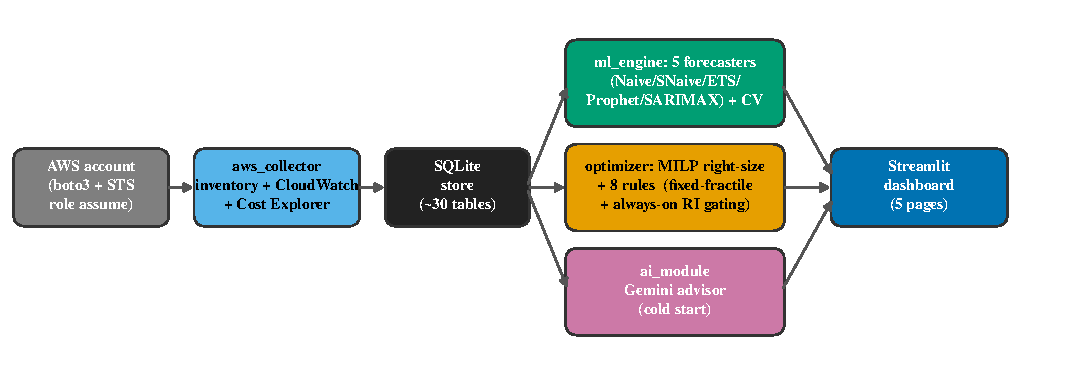
\includegraphics[width=0.92\textwidth]{fig_architecture.pdf}
\caption{Smart Cloud Optimizer architecture. The evaluated research behavior
is the right-sizing and reservation-policy logic, not dashboard presentation
or LLM-advisor output.}
\label{fig:arch}
\end{figure}

\subsection{Forecasting and Monitoring}

The forecasting module exposes a shared fit/predict interface for Naive,
SeasonalNaive, ETS, Prophet, and SARIMAX-style models. The paper scripts
report walk-forward MAPE and selected paired tests where enough aligned
errors are available. Forecasts are used as monitoring context. They are not
the source of the reported right-sizing savings.

\subsection{MILP Right-Sizing}

For compute resources, the optimizer solves a binary assignment problem. Let
$\mathcal{I}$ be resources and $\mathcal{C}$ candidate instance types with
price $p_c$, vCPUs $v_c$, and memory $m_c$. The decision variable
$x_{i,c}\in\{0,1\}$ assigns resource $i$ to candidate $c$:
\begin{align}
\min_x \quad & \sum_{i\in\mathcal{I}}\sum_{c\in\mathcal{C}} p_c x_{i,c}\\
\mathrm{s.t.}\quad & \sum_c x_{i,c}=1 && \forall i,\\
& \sum_c v_c x_{i,c}\ge r_i^{cpu} && \forall i,\\
& \sum_c m_c x_{i,c}\ge r_i^{mem} && \forall i,\\
& \sum_{i,c} p_c x_{i,c}\le B && \mathrm{if\ a\ cap\ is\ supplied}.
\end{align}
EC2 uses CPU and memory when memory utilization is available. RDS uses CPU
because the stored RDS memory metric is not directly comparable as a
utilization percentage.

\subsection{Rules and Reservation Checks}

The rule engine adds transparent service-specific actions such as EC2/RDS
reserved-pricing switches and waste-removal checks. These rules provide
implementation context and a sanity check on the committed demo database.
The paper's quantitative claims come from the generated MILP evidence tables,
the restored public-trace study, and reservation-policy simulations.

\subsection{Price-Basis Normalization}

Price comparability is central to the evaluated evidence. The committed
synthetic database contains EC2 current-inventory costs that mostly match the
2026-06-30 AWS Price List snapshot for Linux, shared-tenancy instances in
\texttt{us-east-1}, but several EC2 candidate rows are incorrect or
incomplete. Therefore, the analysis does not use the stale stored
\texttt{recommendations} table as a headline result. Instead, EC2 current
inventory and EC2 candidates are normalized to the same snapshot on-demand
basis. Two current \texttt{m5.xlarge} rows that were originally recorded at
one-year reserved-instance prices are evaluated on the shared on-demand basis
for right-sizing comparability. This does not mean those instances would be
billed as on-demand in a live account. Reserved-instance and other commitment
effects are evaluated separately through the paper-side usage-hour RI replay
and Study III.

RDS remains on the committed demo database price basis because the paper-local
snapshot covers EC2 only. Consequently, the Study I aggregate result must
always be read with the EC2/RDS split.

\section{Experimental Design}

\subsection{Research Questions}

The evaluation addresses four questions:

\begin{itemize}
\item RQ1: What does the implemented optimizer report on the repository's
synthetic AWS account after repairing the EC2 price basis?
\item RQ2: What mapped-cost changes does the same MILP right-sizing rule
produce on restored public VM traces under a consistent price catalog?
\item RQ3: What do walk-forward MAPE and selected paired tests show about the
forecasting models as monitoring context?
\item RQ4: What is the held-out cost of counterfactually reusing a
high-headroom right-sizing fractile for reservation sizing?
\end{itemize}

\subsection{Datasets and Inputs}

Table~\ref{tab:datasets} summarizes the evaluated inputs. Study I uses the
committed synthetic AWS account. Study II uses restored Bitbrains and Materna
GWA traces~\cite{shen2015bitbrains,iosup2008gwa}, priced against a
snapshot-dated AWS catalog. The Azure Public Dataset V2 arm is retained only
as a generated boundary condition because the raw \texttt{vmtable.csv.gz}
input was not restored in this workspace.

The study uses the GWA fastStorage, GWA Rnd, and GWA Materna traces; the
retained Azure aggregate artifact; synthetic account data; the documented AWS
price/catalog snapshot; and the derived evidence files recorded in the
repository. For the synthetic-account arm, publicly available workload traces
and catalog artifacts were processed and organized into a unified synthetic
account-level environment with generated resource identifiers. The workloads
were assigned across a deliberately complex EC2/RDS-style infrastructure to
support controlled evaluation of the implemented optimization workflow. The
environment simulates selected structural characteristics of an AWS account
but is not a live production account and contains no customer or personal
data. The resulting account-level data are synthetic; they are not output from
AWS, Azure, or another commercial recommender.

\FloatBarrier
\begin{table*}[t]
\caption{Evaluation inputs and artifact status. GWA checksums and provenance
are recorded in \texttt{paper/trace\_provenance.md}; the Azure raw-input
checksum is unavailable because \texttt{vmtable.csv.gz} was not restored.}
\label{tab:datasets}
\centering
\footnotesize
\renewcommand{\arraystretch}{1.08}
\setlength{\tabcolsep}{4pt}
\begin{tabularx}{\textwidth}{@{}>{\raggedright\arraybackslash}p{0.17\textwidth} >{\raggedright\arraybackslash}p{0.18\textwidth} Y Y@{}}
\toprule
Input & Scale and period & Used for & Artifact files \\
\midrule
Synthetic AWS account & \nDays{} days (\dataStart--\dataEnd), \numResources{} resources & optimizer savings, forecasting, policy simulation & \path{paper/results_baselines.json}; \path{paper/results_ablations.json}; \path{paper/numbers_evidence.tex} \\
Bitbrains fastStorage & \extFsVms{} VMs, 2013 trace & real-trace MILP right-sizing & \path{paper/results_external.json}; \path{paper/trace_provenance.md} \\
Bitbrains Rnd & \extRndVms{} VMs, \extRndHours{} hourly aggregate points & right-sizing, forecasting, policy simulation & \path{paper/trace_rnd_hourly.csv}; \path{paper/results_policy_ext.json} \\
Materna-Trace-3 & \extMatVms{} VMs, 2016 trace & second-provider right-sizing validation & \path{paper/results_external.json}; \path{paper/table_external_baselines.tex} \\
Azure Public Dataset V2 & \azVms{} filtered VMs from \azTotalRows{} rows, 2019 trace & recorded boundary case & \path{paper/results_azure.json}; raw input not restored \\
\bottomrule
\end{tabularx}
\end{table*}

\subsection{Metrics and Baselines}

Right-sizing results are reported as estimated monthly cost changes relative
to the relevant baseline. Study I compares the current synthetic inventory
against generated sizing policies. Study II compares each real-trace mapping
against the cheapest AWS type that covers provisioned cores and memory.
Forecasting reports walk-forward MAPE and selected paired-test results where
aligned errors are available. Study III reports held-out policy cost as a
percentage of an on-demand-only baseline.

Study I confidence intervals use 5,000 paired resource-level bootstrap
resamples over the 10 compute resources with seed 20260709. Study II uses
2,000 paired VM-level bootstrap resamples with the same seed. These intervals
describe heterogeneity across the evaluated resources under the fixed price
mapping; they are not population-level confidence statements. Policy replay
is deterministic for a fixed chronological split and is supplemented by
50/60/70\% split sensitivity rather than confidence intervals.

The baseline families are intentionally separated. Mean, median, percentile,
and max right-sizing rows are mathematical baselines. Newsvendor, SAA,
dual-capacity, and recency-window replay rows are paper-side reservation
simulations. The synthetic usage-hour RI replay and Study III recency-window
rows are not AWS Compute Optimizer, Cost Explorer, Azure Advisor, Savings
Plans, or third-party recommender outputs.

\section{Study I: Synthetic Account, Catalog Audit, and Service Decomposition}
\label{sec:study1}

\subsection{Catalog Audit and Feasibility Boundary}

The synthetic account spans \nDays{} days from \dataStart{} to \dataEnd{}.
The pricing audit shows that the committed EC2 current-inventory costs mostly
match the snapshot AWS catalog, but several committed EC2 candidate rows are
wrong or incomplete. The original demo candidate set contains 13 EC2 price
rows, but only four EC2 rows have the positive price and hardware
specifications required by the MILP. Under $q_{0.95}\times1.3$, the EC2
subproblem is therefore partial/infeasible in the original demo catalog while
RDS remains feasible. This is a catalog-completeness boundary, not a
universal claim about P95 sizing.

Table~\ref{tab:catalog-comparison} shows the normalized comparison. With a
shared 28-type EC2 snapshot catalog, non-budget EC2 infeasibilities disappear.
The remaining EC2 infeasibilities are confined to explicit budget-cap rows.

% Journal-only layout of the unchanged generated table values.
\begin{table*}[t]
\caption{Catalog-comparison rerun for the synthetic-account EC2 feasibility
boundary. The snapshot row uses a shared EC2 price basis: current EC2
inventory and EC2 candidates are repriced with the documented AWS Price List
snapshot in \texttt{paper/aws\_catalog.py}; RDS candidates remain from the
committed demo database. The 19.0\% snapshot-row saving is the service-mixed
aggregate decomposed in Table~\ref{tab:service-decomp}. Non-cap EC2 infeasible
rows exclude explicit budget-cap constraints. Partial rows are not comparable
savings estimates.}
\label{tab:catalog-comparison}
\centering
\footnotesize
\renewcommand{\arraystretch}{1.12}
\setlength{\tabcolsep}{2.5pt}
\begin{tabularx}{\textwidth}{@{}Y r r Y r r >{\centering\arraybackslash}p{0.09\textwidth} >{\centering\arraybackslash}p{0.09\textwidth} Y@{}}
\toprule
Catalog/basis & \shortstack{EC2\\raw} & \shortstack{EC2\\valid} &
\shortstack{P95 \(\times\) 1.3\\status} & \shortstack{Cost\\(\$/mo)} &
\shortstack{Saving\\(\%)} & \shortstack{Non-cap\\infeas.\\rows} &
\shortstack{Cap\\infeas.\\rows} & Boundary \\
\midrule
Original demo DB & 13 & 4 & Partial (EC2 Infeasible) & -- & -- & 9/18 & 4/4 &
catalog coverage \\
AWS snapshot shared EC2 basis & 28 & 28 & Optimal & 1,006 & 19.0 & 0/18 & 4/4 &
service budget cap \\
\bottomrule
\end{tabularx}
\vspace{0.25em}
\begin{minipage}{0.98\textwidth}
\footnotesize
EC2 infeasibility disappears for non-budget baseline and ablation rows with
the shared-basis snapshot EC2 catalog; remaining EC2 infeasibility is confined
to explicit per-service budget-cap rows.
\end{minipage}
\end{table*}

\subsection{Baseline and Service-Level Results}

Table~\ref{tab:baselines} reports the generated synthetic baseline grid. The
headline Study I row is the deployed $q_{0.95}\times1.3$ policy on the shared
EC2 snapshot basis. Current synthetic compute cost is
\$\evidComputeCurrent{}/mo and the feasible P95 x 1.3 row costs
\$\evidPfiveCost{}/mo, a compute-scope change of \evidAggregateDeltaPct\%.

\begin{table*}[t]
\caption{Generated synthetic-account baseline comparison. Synthetic compute
rows use a shared price basis: EC2 current
inventory and EC2 candidates are repriced with the snapshot-dated AWS catalog
in \texttt{paper/aws\_catalog.py}; RDS remains on the committed demo DB basis.
Partial or failed rows are not comparable savings estimates and are shown as
``--''.}
\label{tab:baselines}
\centering
\small
\renewcommand{\arraystretch}{1.08}
\setlength{\tabcolsep}{3.5pt}
\begin{tabular}{@{}l r r r r r r l@{}}
\toprule
Method & Resources & Cost & Saving & 95\% CI & Down & Up & Status \\
 & & (\$/mo) & (\%) & (\%) & & & \\
\midrule
Current inventory & 10 & 1,242 & 0.0 & [0.0, 0.0] & 0 & 0 & Baseline \\
Mean utilization & 10 & 347 & 72.0 & [48.0, 85.5] & 9 & 0 & Optimal \\
Median utilization & 10 & 332 & 73.3 & [50.5, 86.4] & 9 & 0 & Optimal \\
P90 sizing & 10 & 660 & 46.8 & [17.5, 74.9] & 9 & 0 & Optimal \\
P95 sizing & 10 & 660 & 46.8 & [17.5, 74.9] & 9 & 0 & Optimal \\
P95 x 1.3 heuristic & 10 & 1,006 & 19.0 & [-48.0, 72.5] & 8 & 2 & Optimal \\
P99 sizing & 10 & 660 & 46.8 & [17.5, 74.9] & 9 & 0 & Optimal \\
Max utilization & 10 & 736 & 40.7 & [10.3, 69.2] & 7 & 0 & Optimal \\
\bottomrule
\end{tabular}
\end{table*}

Table~\ref{tab:service-decomp} is the required interpretation of that
aggregate. EC2 increases from \$\evidEcTwoCurrent{}/mo to
\$\evidEcTwoOptimized{}/mo, a \$\evidEcTwoDelta{}/mo
(\evidEcTwoDeltaPct\%) increase. RDS decreases from
\$\evidRdsCurrent{}/mo to \$\evidRdsOptimized{}/mo, a
\$\evidRdsSavings{}/mo (\evidRdsSavingsPct\%) decrease. Because RDS remains
demo-priced, the aggregate \evidAggregateDeltaPct\% result is
method-illustrative. It is not an unqualified optimizer win and should not be
read as production-dollar evidence.

\begin{table}[t]
\caption{Study I service-level decomposition for the generated $q_{0.95}\times1.3$ row. EC2 current inventory and candidates use the shared snapshot on-demand basis; RDS remains on the committed demo DB basis. Positive deltas indicate cost increases.}
\label{tab:service-decomp}
\centering
\renewcommand{\arraystretch}{1.06}
\begin{tabular}{@{}l r r r r@{}}
\toprule
Scope & Current & Optimized & Delta & Delta \\
 & (\$/mo) & (\$/mo) & (\$/mo) & (\%) \\
\midrule
EC2 & 844 & 971 & +127 & +15.0 \\
RDS & 398 & 35 & -363 & -91.2 \\
Aggregate & 1,242 & 1,006 & -236 & -19.0 \\
\bottomrule
\end{tabular}
\end{table}


The P95 x 1.3 aggregate bootstrap interval,
$[-48.0\%,72.5\%]$, spans both cost increase and cost reduction. Its width is
expected for only 10 heterogeneous resources and a service mix in which the
EC2 and RDS effects have opposite signs. The point estimate is therefore a
transparent case-study summary, not evidence that the same aggregate saving
would generalize to a production fleet.

\subsection{Ablations, Runtime, and Rule Sanity Checks}

Table~\ref{tab:ablations} reports the full synthetic ablation grid. The
percentile and headroom rows show a mapped-cost/headroom tradeoff: lower
requirements can produce higher apparent mapped savings, while P95 x 1.3
selects more candidate capacity. These rows do not measure operational
performance effects. The table also keeps
budget infeasibilities visible rather than converting fallback diagnostics
into comparable savings.

% Journal-only layout of the unchanged generated table values.
\begin{table*}[t]
\caption{Generated ablation results on the synthetic account with EC2 repriced
to the snapshot AWS catalog. Percentile, headroom, memory, and budget rows
report assignment cost only for feasible MILP solves; aggregate 19.0\% rows
inherit the EC2/RDS split and RDS demo-price caveat in
Table~\ref{tab:service-decomp}. Partial or failed rows expose feasibility
limits and are not comparable savings estimates. Rule-set rows are a
recomputed implementation sanity check on the committed demo DB, not the
source of headline paper savings.}
\label{tab:ablations}
\centering
\footnotesize
\renewcommand{\arraystretch}{1.08}
\setlength{\tabcolsep}{3pt}
\begin{tabularx}{\textwidth}{@{}>{\raggedright\arraybackslash}p{0.15\textwidth} Y r r r r >{\raggedright\arraybackslash}p{0.23\textwidth}@{}}
\toprule
Dimension & Level & \shortstack{Cost\\(\$/mo)} &
\shortstack{Saving\\(\%)} & \shortstack{CPU exceed\\(\%)} & Recs/vars & Status \\
\midrule
percentile q & 0.75 & 478 & 61.5 & 1.2 & 232 & Optimal \\
percentile q & 0.90 & 1,006 & 19.0 & 0.0 & 232 & Optimal \\
percentile q & 0.95 & 1,006 & 19.0 & 0.0 & 232 & Optimal \\
percentile q & 0.99 & 1,141 & 8.1 & 0.0 & 232 & Optimal \\
headroom h & 1.0 & 660 & 46.8 & 0.0 & 232 & Optimal \\
headroom h & 1.1 & 660 & 46.8 & 0.0 & 232 & Optimal \\
headroom h & 1.3 & 1,006 & 19.0 & 0.0 & 232 & Optimal \\
headroom h & 1.5 & 1,141 & 8.1 & 0.0 & 232 & Optimal \\
memory constraint & off & 585 & 52.9 & 0.0 & 232 & Optimal \\
memory constraint & observed & 1,006 & 19.0 & 0.0 & 232 & Optimal \\
budget cap & none & 1,006 & 19.0 & 0.0 & 232 & Optimal \\
budget cap & 100\% current & -- & -- & -- & 232 & Partial (EC2 Infeasible) \\
budget cap & 90\% current & -- & -- & -- & 232 & Partial (EC2 Infeasible) \\
budget cap & 75\% current & -- & -- & -- & 232 & Partial (EC2 Infeasible) \\
budget cap & 1\% current & -- & -- & -- & 232 &
Failed (EC2 Infeasible, RDS Infeasible) \\
\midrule
rule set & MILP right-sizing only & -- & -- & -- & 2 & \$362.81/mo \\
rule set & reserved pricing only & -- & -- & -- & 2 & \$125.85/mo \\
rule set & waste rules only & -- & -- & -- & 11 & \$19.17/mo \\
rule set & all rules, deduplicated & -- & -- & -- & 15 & \$507.83/mo \\
\bottomrule
\end{tabularx}
\end{table*}

Table~\ref{tab:runtime} records runtime and clone-stress diagnostics for the
generated evidence script. These are not a hardware-normalized scalability
study, but they document solver status, solve counts, and EC2 MILP stress
sizes used by the current artifact.

% Journal-only layout of the unchanged generated table values.
\begin{table*}[t]
\caption{Runtime and clone-stress diagnostics for the generated evidence
script. GWA Bitbrains/Materna raw-trace parsing runtimes are recorded in
\texttt{paper/trace\_provenance.md}; Azure raw parsing runtime was not
recorded because \texttt{vmtable.csv.gz} was not restored. These diagnostics are not a
hardware-normalized scalability study.}
\label{tab:runtime}
\centering
\small
\renewcommand{\arraystretch}{1.08}
\setlength{\tabcolsep}{4pt}
\begin{tabularx}{\textwidth}{@{}Y r r r r r l@{}}
\toprule
Experiment & \(n\) & Vars & Solves & Solve s & Peak MB & Status \\
\midrule
baseline sweep & 10 & 1624 & 14 & 0.117 & 114.1 & computed \\
ablation sweep & 10 & 3480 & 30 & 0.248 & 118.6 & computed \\
rule-set ablation & 10 & 0 & 0 & 0.557 & 118.6 & computed \\
EC2 MILP stress n=100 & 100 & 2800 & 1 & 0.071 & 120.4 & Optimal \\
EC2 MILP stress n=500 & 500 & 14000 & 1 & 0.396 & 141.5 & Optimal \\
EC2 MILP stress n=1000 & 1000 & 28000 & 1 & 1.285 & 171.4 & Optimal \\
evidence script total & 10 & 49904 & 47 & 7.860 & 171.4 & computed \\
\bottomrule
\end{tabularx}
\end{table*}

The recomputed implementation sanity check emits \evidRuleRecs{} deduplicated
recommendations worth \$\evidRuleSavings{}/mo under the committed demo
database path. This is retained as system-context evidence only. The stale
stored 19-row recommendation table is not used as a headline result.

Table~\ref{tab:ri-replay} reports the paper-side synthetic EC2 usage-hour RI
replay baseline. The 7-, 30-, and 60-day windows collapse to the same row
because the same six eligible on-demand EC2 instances have complete metric
coverage in every window and the snapshot reserved/on-demand prices are
static. This table is not third-party recommender output.

\begin{table}[t]
\caption{Paper-side EC2 usage-hour RI replay baseline. The replay uses trailing observed metric coverage and the same snapshot EC2 on-demand/reserved prices; it is not AWS Compute Optimizer, Cost Explorer, Azure Advisor, or third-party recommender output. The 7-, 30-, and 60-day windows collapse to one row because they select the same six fully observed synthetic EC2 instances.}
\label{tab:ri-replay}
\centering
\renewcommand{\arraystretch}{1.06}
\begin{tabular}{@{}l r r r r l@{}}
\toprule
Recency windows & Recs & Current & Saving & Saving & Status \\
(days) & & (\$/mo) & (\$/mo) & (\%) & \\
\midrule
7/30/60 & 6 & 563 & 209 & 37.1 & paper-side replay \\
\bottomrule
\end{tabular}
\end{table}


\subsection{Synthetic Forecasting Context}

Forecasting is useful for monitoring, but not decisive for the cost claims.
Table~\ref{tab:mape} shows walk-forward MAPE on the synthetic account. ETS has
the best 30-day mean (\mapeEts\%), but the ETS versus seasonal-naive
difference is not statistically significant at the reported sample size
($p=\dmPEtsSnaive$). The paper therefore treats ETS as a selected monitoring
model, not proof of forecast-driven optimization superiority.

\begin{table*}[t]
\caption{Study I synthetic-account walk-forward MAPE (\%, mean $\pm$ sd).
Values are transcribed unchanged from the table generated by
\texttt{paper/make\_figures.py}.}
\label{tab:mape}
\centering
\small
\renewcommand{\arraystretch}{1.10}
\setlength{\tabcolsep}{3pt}
\begin{tabularx}{\textwidth}{@{}l *{5}{Z}@{}}
\toprule
Model & \(h{=}7\) & \(h{=}14\) & \(h{=}30\) & \(h{=}60\) & \(h{=}90\) \\
\midrule
ETS (selected) & 11.28 \(\pm\) 2.54 & 11.24 \(\pm\) 2.45 &
\textbf{11.20 \(\pm\) 0.57} & \textbf{11.39 \(\pm\) 0.74} &
\textbf{12.15 \(\pm\) 2.39} \\
SeasonalNaive & \textbf{10.18 \(\pm\) 2.84} &
\textbf{10.84 \(\pm\) 2.75} & 12.28 \(\pm\) 2.82 &
12.66 \(\pm\) 2.21 & 12.91 \(\pm\) 2.02 \\
Prophet & 14.41 \(\pm\) 6.22 & 20.47 \(\pm\) 7.40 &
20.93 \(\pm\) 7.53 & 19.70 \(\pm\) 7.89 & 18.08 \(\pm\) 8.42 \\
Naive & 25.16 \(\pm\) 4.47 & 27.90 \(\pm\) 3.52 &
27.26 \(\pm\) 4.36 & 27.87 \(\pm\) 4.09 & 27.38 \(\pm\) 3.70 \\
\bottomrule
\end{tabularx}
\end{table*}

\FloatBarrier

\section{Study II: Restored GWA Real-Trace Validation}
\label{sec:study2}

\subsection{Restoration and Cost Model}

Study II was restored and rerun from raw GWA inputs. The artifact records
archive-content SHA256 hashes for the Bitbrains fastStorage zip, Bitbrains Rnd
zip, and Materna zip, plus filename-and-size manifest SHA256 hashes for the
extracted CSV trees. The rerun uses a
snapshot-dated AWS EC2 catalog from \extSnapshot{} with \extCatalogSize{}
candidate types. Each VM baseline maps provisioned cores and memory to the
cheapest covering AWS type. The optimized assignment uses the same deployed
$q_{0.95}\times1.3$ requirement.

Table~\ref{tab:gwa-provenance} summarizes the restored inputs. It reports
16-hex prefixes for readability; the complete archive-content and
filename-and-size manifest SHA256 values are preserved in
\path{paper/trace_provenance.md} and \path{paper/results_external.json}.

\begin{table*}[t]
\caption{Restored GWA provenance summary. Archive hashes cover archive
contents; manifest hashes cover only relative filenames/paths and file sizes.
The 1,500 Rnd CSV files represent the same 500 VMs across three monthly
directories. The Materna archive contains 1,593 CSV files; the evaluation uses
547 VMs from Trace~3.}
\label{tab:gwa-provenance}
\centering
\small
\renewcommand{\arraystretch}{1.08}
\begin{tabular}{@{}l r r l l@{}}
\toprule
Archive & Bytes & Extracted CSVs & Archive SHA256 prefix &
\shortstack{Filename/size manifest\\SHA256 prefix} \\
\midrule
fastStorage & 134,047,207 & 1,250 & \texttt{11313f528a0cbcbe} & \texttt{63e26df5c3af611b} \\
Rnd & 163,099,172 & 1,500 & \texttt{d3d9ddebb689c0b5} & \texttt{5e288d1ae5c7cb8e} \\
Materna & 145,292,565 & 1,593 & \texttt{1380879f0de17cb5} & \texttt{07ff13555d88df59} \\
\bottomrule
\end{tabular}
\end{table*}

The recorded rerun wall times were 176.06 seconds for fetch/extraction,
169.12 seconds for external validation, 127.34 seconds for the checksum,
raw-quantile-scan, and baseline-grid helper stages, and 4.51 seconds for the
real-trace policy simulation. These timings document the artifact run; they
are not a hardware-normalized scalability benchmark; a full
process-memory and dependency-version inventory was not recorded.

The absolute dollar values are mapped costs, not observed AWS bills. The GWA
traces are older managed-hosting traces priced against a 2026 AWS catalog.
The percentages provide within-model comparisons under this shared mapping.

\subsection{Right-Sizing Results with Confidence Intervals}

Table~\ref{tab:external} reports the restored GWA right-sizing results under
the evaluated mapping. On Bitbrains fastStorage and Rnd, the mapped-cost
reductions are \extFsSavingsPct\% (95\% CI
\extFsSavingsCiLow--\extFsSavingsCiHigh\%) and \extRndSavingsPct\%
(\extRndSavingsCiLow--\extRndSavingsCiHigh\%), respectively. On Materna, the
mapped reduction is \extMatSavingsPct\%
(\extMatSavingsCiLow--\extMatSavingsCiHigh\%). Across all restored GWA VMs,
the aggregate mapped reduction is \extOverallSavingsPct\%
(\extOverallSavingsCiLow--\extOverallSavingsCiHigh\%). Applying one-year
reserved pricing to the optimized always-on fleet raises the aggregate mapped
reduction to \extOverallSavingsPctRi\%
(\extOverallSavingsPctRiCiLow--\extOverallSavingsPctRiCiHigh\%).

\begin{table}[t]
\caption{Study II restored-GWA right-sizing at AWS on-demand rates from
snapshot \extSnapshot. The $+$RI column applies one-year reserved pricing.}
\label{tab:external}
\centering
\renewcommand{\arraystretch}{1.08}
\setlength{\tabcolsep}{3.5pt}
\begin{tabular}{@{}l r r r r@{}}
\toprule
Dataset & VMs & Baseline & Optimized & Saving / $+$RI \\
 & & (\$/mo) & (\$/mo) & (\%) \\
\midrule
fastStorage & \extFsVms{} & \extFsBaseline{} & \extFsOptimized{} & \extFsSavingsPct{} / \extFsSavingsPctRi{} \\
Rnd & \extRndVms{} & \extRndBaseline{} & \extRndOptimized{} & \extRndSavingsPct{} / \extRndSavingsPctRi{} \\
Materna & \extMatVms{} & \extMatBaseline{} & \extMatOptimized{} & \extMatSavingsPct{} / \extMatSavingsPctRi{} \\
\bottomrule
\end{tabular}
\end{table}

\subsection{Full Baseline Grid and Mapped-Cost/Headroom Interpretation}

Table~\ref{tab:external-baselines-full} gives the full restored-GWA baseline
grid with costs and bootstrap intervals. Mean, median, and less-conservative
percentile sizing can produce higher apparent mapped savings than
$q_{0.95}\times1.3$. These rows are not automatically better policies because
the repository does not evaluate SLO, latency, error, throughput, availability,
or other operational outcomes after right-sizing. The table exposes a
mapped-cost/headroom tradeoff: P95 x 1.3 selects larger candidate capacities
and yields lower mapped savings than several rows. Added headroom is not
evidence of operational performance safety.

\begin{table*}[t]
\caption{Full Study II restored-GWA baseline grid. Savings are relative to the
lift-and-shift mapping and include bootstrap 95\% intervals.}
\label{tab:external-baselines-full}
\centering
\small
\renewcommand{\arraystretch}{1.04}
\setlength{\tabcolsep}{3pt}
% Auto-generated by paper/study2_reproducibility.py -- do not edit by hand.
\begin{tabular}{@{}l l r r@{}}
\toprule
Dataset & Policy & Cost (\$/mo) & Saving [95\% CI] \\
\midrule
fastStorage & Lift-and-shift & 128,588 & 0.0 [0.0, 0.0] \\
fastStorage & Mean & 23,920 & 81.4 [79.0, 83.6] \\
fastStorage & Median & 16,973 & 86.8 [85.0, 88.3] \\
fastStorage & P90 & 68,673 & 46.6 [38.8, 53.9] \\
fastStorage & P95 & 76,845 & 40.2 [32.0, 48.0] \\
fastStorage & P99 & 84,908 & 34.0 [25.6, 41.8] \\
fastStorage & Max & 119,196 & 7.3 [-1.1, 15.4] \\
fastStorage & P95 x 1.3 & 85,414 & 33.6 [24.5, 41.8] \\
Rnd & Lift-and-shift & 44,294 & 0.0 [0.0, 0.0] \\
Rnd & Mean & 7,728 & 82.6 [79.4, 85.5] \\
Rnd & Median & 4,273 & 90.4 [88.7, 91.9] \\
Rnd & P90 & 25,697 & 42.0 [28.6, 54.3] \\
Rnd & P95 & 27,720 & 37.4 [23.5, 50.3] \\
Rnd & P99 & 30,088 & 32.1 [17.9, 45.0] \\
Rnd & Max & 45,947 & -3.7 [-18.8, 10.6] \\
Rnd & P95 x 1.3 & 29,614 & 33.1 [19.3, 46.3] \\
Materna & Lift-and-shift & 44,184 & 0.0 [0.0, 0.0] \\
Materna & Mean & 6,141 & 86.1 [84.7, 87.3] \\
Materna & Median & 5,974 & 86.5 [85.1, 87.7] \\
Materna & P90 & 8,223 & 81.4 [79.4, 83.2] \\
Materna & P95 & 9,370 & 78.8 [76.5, 80.9] \\
Materna & P99 & 11,786 & 73.3 [70.5, 75.9] \\
Materna & Max & 25,300 & 42.7 [38.3, 47.3] \\
Materna & P95 x 1.3 & 11,398 & 74.2 [71.4, 76.8] \\
\bottomrule
\end{tabular}

\end{table*}

\subsection{Azure Boundary Condition}

The Azure Public Dataset V2 result is retained as a boundary condition, not as
a rerun claim. The raw \texttt{vmtable.csv.gz} file was not present in this
workspace, so the Azure arm was not restored, checksummed, rerun, or extended
with confidence intervals. The committed generated artifact contains
\azVms{} filtered VMs from \azTotalRows{} rows. Under the recorded Azure
preprocessing and metric-semantics assumptions, the mapped right-sizing result
was \azSavingsPct\%, while the recorded result with reserved pricing was
\azSavingsPctRi\%. Because the raw Azure input was not restored and those
assumptions were not independently ablated, this result identifies a boundary
case but does not establish which assumption caused the reversal.

\subsection{Real-Trace Forecasting Context}

Table~\ref{tab:extmape} reports the Rnd aggregate forecast errors, and
Figure~\ref{fig:ext-series} shows the series used for forecasting and policy
replay. Forecasting the real aggregate is difficult. At 24 hours, the best hourly model is
\extBestModel{} with \extBestMape\% MAPE, and tested pairwise differences are
not statistically significant (for example, ETS vs. seasonal-naive
$p=\extDmP$). The evidence supports treating forecasts as monitoring context
rather than the source of right-sizing savings.

\begin{table*}[t]
\caption{Study II real Rnd aggregate forecasting MAPE (\%, mean $\pm$ sd).}
\label{tab:extmape}
\centering
\footnotesize
\renewcommand{\arraystretch}{1.08}
\setlength{\tabcolsep}{2.5pt}
\begin{tabularx}{\textwidth}{@{}l *{6}{Z}@{}}
\toprule
Model & \(h{=}6\)\,h & \(h{=}12\)\,h & \(h{=}24\)\,h &
\(h{=}48\)\,h & \(h{=}7\)\,d & \(h{=}14\)\,d \\
\midrule
ETS & \textbf{48.2 \(\pm\) 46.2} & 71.9 \(\pm\) 55.4 &
77.0 \(\pm\) 57.2 & 91.2 \(\pm\) 47.8 &
\textbf{52.1 \(\pm\) 29.9} & 64.4 \(\pm\) 40.9 \\
SeasonalNaive & 65.9 \(\pm\) 33.6 & 73.7 \(\pm\) 46.3 &
65.0 \(\pm\) 40.3 & \textbf{65.8 \(\pm\) 33.8} &
54.2 \(\pm\) 22.6 & \textbf{59.7 \(\pm\) 32.9} \\
Prophet & 49.0 \(\pm\) 26.2 & \textbf{60.5 \(\pm\) 30.0} &
\textbf{60.8 \(\pm\) 21.6} & 88.1 \(\pm\) 42.3 &
59.8 \(\pm\) 36.9 & 66.7 \(\pm\) 30.0 \\
Naive & 57.4 \(\pm\) 71.2 & 87.9 \(\pm\) 86.1 &
82.3 \(\pm\) 66.6 & 94.2 \(\pm\) 55.7 &
53.4 \(\pm\) 14.2 & 66.5 \(\pm\) 44.5 \\
\bottomrule
\end{tabularx}
\end{table*}

\begin{figure}[t]
\centering
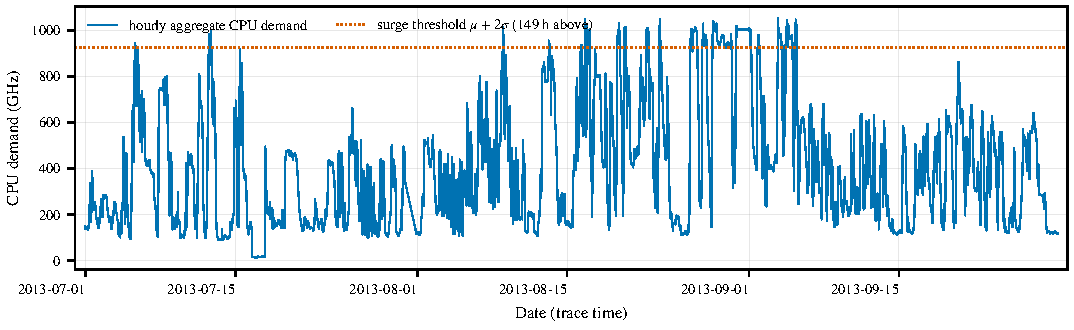
\includegraphics[width=0.92\textwidth]{fig_ext_series.pdf}
\caption{Bitbrains Rnd aggregate demand series used for real-trace
forecasting context and Study III policy replay.}
\label{fig:ext-series}
\end{figure}

\section{Study III: Capacity-Reservation Policy Simulation}
\label{sec:study3}

\subsection{Protocol}

Study III isolates the reservation-sizing question. Each simulation splits an
empirical proxy series \(X_t\) chronologically into train and test segments,
selects a commitment proxy \(Q\) from the training data, and charges that
policy on the held-out suffix. The synthetic run uses \polTrainPeriods{}
training days and \polTestPeriods{} test days. The restored real-trace run
uses \extPolTrainPeriods{} training hours and \extPolTestPeriods{} test hours
from the Bitbrains Rnd aggregate.

The deployed $q_{0.95}\times1.3$ right-sizing rule is reused
counterfactually as a naive reservation-sizing rule. This is neither deployed
reservation behavior nor a model of AWS, Azure, or commercial recommendation
systems. The counterfactual quantifies mapped cost when the algebra of a
high-headroom sizing rule is applied to a commitment-proxy decision.

\subsection{Empirical Mapping and Units}

The theoretical formulation in Section~3 expresses \(D_t\) and \(K\) in
physical-capacity units. The empirical simulations preserve the objective's
algebra but use arm-specific quantities \(X_t\) and \(Q\) to avoid implying
that both inputs are physical capacity. In the synthetic arm, \(X_t\) is the
daily account-cost series read from \texttt{total\_cost}; both \(X_t\) and
\(Q\) are measured in USD/day. This arm evaluates relative temporal policy
behavior on a cost-proxy time series. It does not simulate provider billing or
physical-capacity allocation directly.

In the restored real-trace arm, \(X_t\) is the hourly aggregate CPU demand
constructed by summing per-VM hourly-mean CPU use, and \(X_t\) and \(Q\) are
measured in MHz. The objective then has on-demand-rate-normalized,
MHz-equivalent mapped-cost units per hourly period; it is not an observed
cloud bill or a resource-level allocation simulation. Reported percentages
divide each arm's mapped cost by its own on-demand-only baseline and are
dimensionless. Absolute \(Q\) values and mapped-cost units are not compared
across arms.

For an empirical training sample \(S_X\), the static proxy objective is the
sample analogue of the theoretical model:
\begin{equation}
\widehat C_\gamma(Q;S_X)
  = \gamma Q + \frac{1}{|S_X|}\sum_{x\in S_X}(x-Q)^+ .
\end{equation}
Every non-clairvoyant policy is sized only on the chronological training
prefix and is then charged on the untouched test suffix. The policy set is:
\begin{itemize}
\item \textbf{OD:} on-demand only, \(Q=0\).
\item \textbf{HEUR:} \(Q=1.3q_{0.95}(S_X)\), the deployed right-sizing rule
read counterfactually as proxy commitment sizing.
\item \textbf{NV:} \(Q=q_{1-\gamma}(S_X)\), the empirical newsvendor solution.
\item \textbf{SAA:} a PuLP/CBC linear program that minimizes
\(\widehat C_\gamma\) over the training scenarios. It represents the same
static objective as NV and is used as an implementation cross-check, not as
an independent adversarial baseline.
\item \textbf{LOOK7/30/60:} the NV/SAA objective fitted to only the trailing
7, 30, or 60 days of training data. These are 7/30/60 daily observations in
the synthetic arm and \extPolLookSevenPeriods{}/
\extPolLookThirtyPeriods{}/\extPolLookSixtyPeriods{} hourly observations in
the real-trace arm. If the requested window exceeds the training prefix, the
implementation uses the complete prefix. These rows are paper-side
recency-window baselines, not evidence about recommendation systems.
\item \textbf{DUAL/DUALC:} a two-level SAA with always-reserved base
\(Q_0\), supplementary proxy commitment \(Q_1-Q_0\), and a training threshold
of the mean plus two standard deviations. DUAL observes the contemporaneous
threshold state and is an information-rich comparator; DUALC activates the
same supplementary level from the previous period's threshold signal.
\item \textbf{LB:} The perfect-information lower-bound cost is
\(C_{\mathrm{LB}}=\gamma\mathbb{E}[X_{\mathrm{test}}]\), obtained by allowing a
period-specific proxy commitment \(Q_t=X_t\). Its units are USD/day proxy
units in the synthetic arm and on-demand-rate-normalized MHz-equivalent units
per hourly period in the real-trace arm. The bound is unattainable under
advance commitment because it uses each future \(X_t\) to choose \(Q_t\).
\end{itemize}

\FloatBarrier
\subsection{Synthetic and Real-Trace Proxy Results}

At the evaluated catalog-average ratio $\gamma=\polGammaStar$, the
high-percentile counterfactual realizes
\polPctHeur\% of on-demand cost on the synthetic USD/day proxy and
\extPolPctHeur\% on the real-trace MHz proxy. The newsvendor fractile realizes
\polPctNv\% and \extPolPctNv\%. This is the mapped-cost gap from counterfactually
reusing a high-headroom sizing rule as proxy commitment sizing under the
evaluated model. Table~\ref{tab:policy-star} reports the complete policy
comparison at this ratio.

\begin{table}[t]
\caption{Held-out policy cost at the evaluated catalog-average
\(\gamma=\polGammaStar\), as a percentage of on-demand-only cost. LOOK rows
are recency-window replay baselines; DUAL observes contemporaneous state; LB
is an unattainable perfect-information cost lower bound.}
\label{tab:policy-star}
\centering
\small
\renewcommand{\arraystretch}{1.05}
\begin{tabular}{@{}l r r@{}}
\toprule
Policy & \shortstack{Synthetic\\cost-proxy arm} &
\shortstack{Restored Rnd\\proxy arm} \\
\midrule
On-demand only & 100.0 & 100.0 \\
P95 x 1.3 counterfactual & \polPctHeur{} & \extPolPctHeur{} \\
Newsvendor & \polPctNv{} & \extPolPctNv{} \\
SAA & \polPctSaa{} & \extPolPctSaa{} \\
LOOK7 & \polPctLookSeven{} & \extPolPctLookSeven{} \\
LOOK30 & \polPctLookThirty{} & \extPolPctLookThirty{} \\
LOOK60 & \polPctLookSixty{} & \extPolPctLookSixty{} \\
Dual, observed state & \polPctDual{} & \extPolPctDual{} \\
Dual, lagged signal & \polPctDualc{} & \extPolPctDualc{} \\
Perfect-information bound & \polPctLb{} & \extPolPctLb{} \\
\bottomrule
\end{tabular}
\end{table}

To avoid comparing the price-aware policies only against the deliberately
conservative HEUR counterfactual, we include LOOK7, LOOK30, and LOOK60 as
paper-side recency-window replay baselines. They are not outputs of, or
evidence about, third-party recommendation systems. On the real trace at
$\gamma=\polGammaStar$, the 7-day replay realizes \extPolPctLookSeven\%,
the 30-day replay realizes \extPolPctLookThirty\%, and the 60-day replay
realizes \extPolPctLookSixty\% of on-demand cost. The LOOK60 row equals the
newsvendor row in the real-trace grid because the requested 60-day window
exceeds the available training split; the implementation falls back to the
full training set, making LOOK60 use the same empirical distribution as the
newsvendor policy.

The dual-capacity rows are close to NV on the synthetic daily series and have
lower mapped cost than NV on the real trace under the evaluated simplified
model and price ratios. This observational comparison does not establish why
the difference occurs. The simulation remains an aggregate model, not a full
dynamic $(s,S)$ contract implementation.

The split-sensitivity replay shows how the mapped-cost ordering varies across
alternative chronological splits. Across 50/60/70\% training fractions,
newsvendor
saves \polNvSaveMin--\polNvSaveMax\% on the synthetic series and
\extPolNvSaveMin--\extPolNvSaveMax\% on the real series. The corresponding
HEUR-minus-NV gaps are \polPoCMin--\polPoCMax{} and
\extPolPoCMin--\extPolPoCMax{} on-demand-cost percentage points. These are
deterministic alternative splits, not confidence intervals.

Figure~\ref{fig:policy-curves} shows both proxy-arm policy curves
across the full price-ratio sweep. Tables~\ref{tab:policy-synth}
and~\ref{tab:policy-real} give the exact grid at four representative ratios.

\begin{table}[t]
\caption{Study III synthetic daily cost-proxy results as \% of the
on-demand-only baseline across the price-ratio grid. LOOK rows are paper-side
recency-window baselines.}
\label{tab:policy-synth}
\centering
\renewcommand{\arraystretch}{1.08}
\setlength{\tabcolsep}{4pt}
\begin{tabular}{@{}l r r r r @{}}
\toprule
Policy & $\gamma{=}0.60$ & $\gamma{=}0.70$ & $\gamma{=}0.80$ & $\gamma{=}0.90$ \\
\midrule
P95 $\times$ 1.3 counterfactual & 97.0 & 113.0 & 128.9 & 144.9 \\
newsvendor $1{-}\gamma$ & 70.8 & 79.7 & 87.7 & 94.5 \\
SAA stochastic program & 70.8 & 79.8 & 87.8 & 94.5 \\
7-day recency-window replay & 71.0 & 80.2 & 87.6 & 94.5 \\
30-day recency-window replay & \textbf{70.5} & \textbf{79.7} & \textbf{87.4} & \textbf{94.3} \\
60-day recency-window replay & 70.5 & 79.8 & 87.5 & 94.6 \\
dual $(Q_0,Q_1)$, obs.\ state & 70.0 & 79.2 & 87.3 & 94.2 \\
dual $(Q_0,Q_1)$, lagged signal & 71.8 & 80.6 & 88.8 & 95.7 \\
perfect-information bound & 60.0 & 70.0 & 80.0 & 90.0 \\
\bottomrule
\end{tabular}

\end{table}

\begin{table}[t]
\caption{Study III real-trace hourly CPU-demand-proxy results as \% of the
on-demand-only baseline across the price-ratio grid. LOOK60 degenerates to NV
because it uses the full training prefix.}
\label{tab:policy-real}
\centering
\renewcommand{\arraystretch}{1.08}
\setlength{\tabcolsep}{4pt}
\begin{tabular}{@{}l r r r r @{}}
\toprule
Policy & $\gamma{=}0.60$ & $\gamma{=}0.70$ & $\gamma{=}0.80$ & $\gamma{=}0.90$ \\
\midrule
P95 $\times$ 1.3 counterfactual & 146.2 & 170.6 & 195.0 & 219.3 \\
newsvendor $1{-}\gamma$ & 84.4 & 89.8 & 94.1 & 97.4 \\
SAA stochastic program & 84.4 & 89.8 & 94.1 & 97.4 \\
7-day recency-window replay & 89.3 & 95.6 & 102.4 & 103.6 \\
30-day recency-window replay & 82.7 & 89.2 & 93.8 & 97.3 \\
60-day recency-window replay & 84.4 & 89.8 & 94.1 & 97.4 \\
dual $(Q_0,Q_1)$, obs.\ state & 75.4 & 82.7 & 89.2 & 94.9 \\
dual $(Q_0,Q_1)$, lagged signal & \textbf{75.8} & \textbf{83.1} & \textbf{89.6} & \textbf{95.3} \\
perfect-information bound & 60.0 & 70.0 & 80.0 & 90.0 \\
\bottomrule
\end{tabular}

\end{table}

\FloatBarrier
\begin{figure}[t]
\centering
\begin{minipage}[t]{0.48\textwidth}
\centering
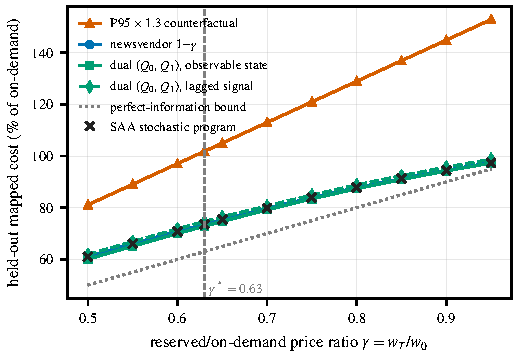
\includegraphics[width=\linewidth]{fig_policy_gamma.pdf}\\[-1mm]
\footnotesize\textbf{(a)} Synthetic daily account-cost proxy (USD/day).
\end{minipage}\hfill
\begin{minipage}[t]{0.48\textwidth}
\centering
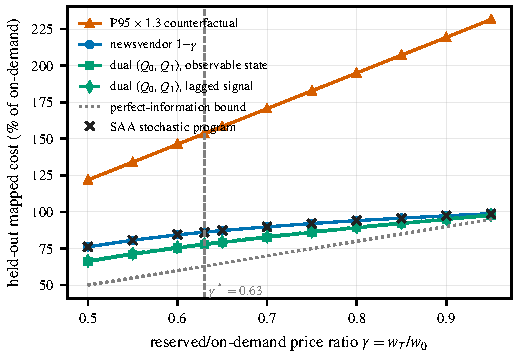
\includegraphics[width=\linewidth]{fig_policy_gamma_ext.pdf}\\[-1mm]
\footnotesize\textbf{(b)} Real-trace hourly aggregate CPU demand (MHz).
\end{minipage}
\caption{Study III held-out mapped cost as a percentage of each arm's
on-demand-only baseline across the price-ratio sweep. At
\(\gamma=\polGammaStar\), the P95 \(\times\) 1.3 counterfactual exceeds the
synthetic baseline and has higher mapped cost than the reported price-aware
policies on both proxy arms. Panel (b)'s dual-level variants have lower mapped
cost than NV on this trace under the simplified model. These curves are not
provider-billing or physical-allocation simulations.}
\label{fig:policy-curves}
\end{figure}

\section{Discussion}

\subsection{What the Evidence Supports}

The evaluated evidence supports three scoped observations. First, the
implemented system operationalizes a percentile-and-headroom rule through MILP
right-sizing and transparent service rules, subject to price-basis and
candidate-catalog feasibility. Second, the documented artifact reruns report
results from the synthetic database, restored public GWA traces, and a
snapshot-dated price catalog. Third, a paper-side simulation that reuses
inherited reservation logic reports different mapped costs for the
high-headroom counterfactual and price-aware policies on two explicitly
labeled proxy series.

The central empirical evidence is the combination of restored GWA
right-sizing with confidence intervals and the held-out reservation-policy
simulation, rather than the synthetic aggregate alone. Study I records
price-basis and catalog-completeness issues in a controlled repository
account. On the restored GWA traces, the same right-sizing rule produced the
reported mapped-cost reductions relative to lift-and-shift under the evaluated
catalog and mapping. Study III reports dimensionless within-arm cost ratios
under the synthetic USD/day cost proxy, the real-trace MHz demand proxy, the
static objective, and the evaluated price ratios. It does not convert either
arm into provider-billing or deployed-allocation evidence.

\subsection{What Should Not Be Oversold}

The deployed system does not implement the full dynamic $(s,S)$ policy of
Chen et al.~\cite{chen2024capacity}. It implements static high-percentile
right-sizing and always-on reserved-pricing checks. The newsvendor, SAA,
dual-level, and recency-window results reuse inherited policy structure in
paper-side simulations; they are not a theoretical extension. The LLM advisor
is not evaluated for savings. The external baselines are mathematical or
replay baselines, not direct runs of AWS, Azure, or third-party recommenders.
The EC2 catalog comparison uses a documented 28-type snapshot, not an all-SKU
AWS catalog.

The prior Azure aggregate remains a boundary case under recorded preprocessing
and metric-semantics assumptions. Without the restored raw input or targeted
ablations, it does not identify the cause of the mapped-cost reversal.

The higher-savings rows in Study II should also not be overread. They may be
lower-cost under the mapping, but the repository does not measure latency,
errors, throughput, availability, or SLO outcomes after right-sizing. The
paper can therefore discuss a mapped-cost/candidate-capacity tradeoff, but it
cannot claim that any row is operationally safe.

\subsection{Implications for Practice}

The practical implication is to separate the modeled decisions and their
evidence. The implemented P95 x 1.3 rule adds capacity headroom and selects
larger candidate sizes under the right-sizing mapping; the study does not
establish whether that headroom improves latency, errors, throughput,
availability, or SLO attainment. The paper-side reservation simulation
separately accounts for the price ratio and proxy-series distribution. Under
the evaluated series and price ratios, counterfactually reusing P95 x 1.3
produced higher mapped cost than the reported price-aware alternatives. That
comparison remains a simulation result, not implemented provider behavior.

\section{Threats to Validity}

\textbf{Synthetic data and demo pricing.} Study I uses the repository's
synthetic AWS account. Its dollar values are method-illustrative and should
not be presented as production savings. The aggregate P95 x 1.3 compute-scope
change is dominated by demo-priced RDS while EC2 increases on the shared
snapshot on-demand basis.

\textbf{Price basis and catalog scope.} EC2 right-sizing rows use a
snapshot-dated 28-type catalog, not an all-SKU AWS catalog and not live AWS
Compute Optimizer output. RDS remains on the committed demo database basis.
Reserved-instance effects are separated from right-sizing.

\textbf{Trace age and provider mapping.} Bitbrains and Materna are older
managed-hosting traces. They are mapped to a 2026 AWS catalog, so percentages
are more defensible than absolute dollar values.

\textbf{Azure raw-input gap.} The Azure result remains a generated boundary
condition because raw \texttt{vmtable.csv.gz} was absent. It needs
restoration, checksum verification, rerun, confidence intervals, and runtime
recording before it can carry the same evidentiary weight as the GWA study.

\textbf{Azure preprocessing and metric semantics.} Under the recorded
assumptions, the Azure mapped result is a boundary case. Because the raw input
was not restored and the assumptions were not independently ablated, the
study cannot attribute the reversal to max-based CPU semantics, unavailable
memory utilization, or any specific preprocessing choice.

\textbf{Policy abstraction and empirical units.} Study III uses a daily
account-cost proxy in USD/day for the synthetic arm and hourly aggregate CPU
demand in MHz for the real-trace arm. Its within-arm percentages are
dimensionless, but its absolute proxy commitments are not comparable across
arms. The simulation does not model provider billing, physical allocation,
all real contract terms, partial upfront payments, cancellation, resale,
family constraints, regional capacity, Savings Plans, or fragmentation.

\textbf{Policy uncertainty.} Study III is deterministic for each
chronological split and reports split sensitivity, but it does not provide
confidence intervals for policy-cost ratios. The dual-state results also
depend on a mean-plus-two-standard-deviations surge threshold and should be
read as model sensitivity rather than a production guarantee.

\textbf{No direct third-party baseline.} The usage-hour RI replay and
recency-window rows are paper-side baselines only. The repository contains no
direct AWS, Azure, or third-party recommender output on the same workload.

\textbf{No SLO or performance-risk validation.} The artifact reports mapped
costs and limited exceedance proxies, but no live SLO, latency, error-rate, or
business-performance outcomes. It therefore cannot claim safe performance
after more aggressive right-sizing.

\textbf{Statistical power.} Forecasting tests use limited walk-forward folds.
Non-significant differences remain non-claims.

\section{Reproducibility and Artifact Availability}

Most headline values are imported from generated artifacts, and the
documented scripts provide rerun paths for the principal synthetic,
restored-GWA, and policy results. Some compact presentation tables contain
transcribed summaries or checksum prefixes. Synthetic evidence is generated
by \path{paper/evidence_experiments.py} and
\path{paper/catalog_comparison.py}; GWA evidence uses
\path{paper/external_validation.py},
\path{paper/study2_reproducibility.py}, and the commands in
\path{paper/trace_provenance.md}; policy results use
\path{paper/policy_sim.py} and \path{paper/trace_rnd_hourly.csv}. The reference
audit in \path{paper/reference_check.md} records that the 23 citation keys used
by the source manuscript resolve. This article uses the same audited key set
and introduces no new bibliography entries.

The principal rerun path is documented, but dependency pinning and independent
clean-room verification are not part of the current artifact. Azure is not
reproducible in this workspace because the raw \texttt{vmtable.csv.gz} input
was not restored. The implementation, generated evidence, build scripts, and
reproducibility materials are maintained in the project repository and are
available from the corresponding author. No public archive DOI has been
assigned. The current artifact does not provide a dependency lock, a complete
environment and execution-hardware inventory, or final generated-file hashes.

\section{Conclusion}

This study contributes an empirical and systems comparison, not new
reservation theory. The implemented behavior is a
\(q_{0.95}\times1.3\) MILP right-sizing pipeline whose reported outcomes
depend on price comparability and candidate-catalog feasibility. On the
synthetic account, the \evidAggregateDeltaPct\% service-mixed change combines
an EC2 increase of \evidEcTwoDeltaPct\% with a demo-priced RDS decrease of
\evidRdsSavingsPct\%. On restored Bitbrains and Materna traces, the same
implemented rule produces \extOverallSavingsPct\% lower mapped cost than
lift-and-shift under the evaluated catalog and mapping (95\% CI
\extOverallSavingsCiLow--\extOverallSavingsCiHigh\%). The Study III results
are separate paper-side simulations that reuse theory-derived logic on a
synthetic USD/day cost proxy and a real-trace MHz demand proxy. They do not
represent provider billing, commercial recommender behavior, or physical
allocation. The Azure arm remains unrestored, and operational performance and
SLO effects remain unresolved.

\section*{Declarations}

\textbf{Funding.} This research received no external funding.

\textbf{Ethics approval.} Not applicable. The study did not involve human
participants, personal data, interviews, surveys, medical information, or
identifiable customer data.

\textbf{Consent to participate.} Not applicable.

\textbf{Consent for publication.} Not applicable.

\textbf{Data availability.} The study uses publicly available workload traces,
pricing and catalog artifacts, and derived synthetic data. The public sources,
checksums, preprocessing procedures, and generated evidence are documented in
the accompanying artifact materials. The workloads were reorganized into a
unified synthetic EC2/RDS-style account environment with generated resource
identifiers. The raw Azure input associated with the retained prior aggregate
result was not restored and is identified as an artifact limitation.

\textbf{Code availability.} The implementation, generated evidence, build
scripts, and reproducibility materials are maintained in the project
repository and are available from the corresponding author.

\textbf{AI-assistance disclosure.} The corresponding author used generative
AI tools for organizing the synthetic infrastructure representation, assigning
processed workloads across EC2-style and RDS-style resources, software
organization, code review, and manuscript presentation. Reported numerical
results were produced by the documented repository workflows. The
corresponding author reviewed and verified the final code, experimental
outputs, numerical values, claims, citations, and manuscript text.

\textbf{Prior dissemination.} An earlier version of this work was prepared as
a university project report. The manuscript has not previously been submitted
to or published by a conference or journal.

\section*{Author Contact Information}
\noindent\textbf{Corresponding author:} Ibrahim Mohamed:
\href{mailto:ibrahimmohamedabdelsadek@gmail.com}{\nolinkurl{ibrahimmohamedabdelsadek@gmail.com}}.

\noindent\textbf{Author emails:} Mariam Emad:
\href{mailto:mariamemadcs@gmail.com}{\nolinkurl{mariamemadcs@gmail.com}}; Hazem Ibrahim:
\href{mailto:Ihazem28@gmail.com}{\nolinkurl{Ihazem28@gmail.com}}; Ahmed Sameh:
\href{mailto:ahmed.sameh.12543@gmail.com}{\nolinkurl{ahmed.sameh.12543@gmail.com}}; Mahmoud Ahmed:
\href{mailto:mahmoudkamel9102003@gmail.com}{\nolinkurl{mahmoudkamel9102003@gmail.com}}; John Ehab:
\href{mailto:ehabjohn22@gmail.com}{\nolinkurl{ehabjohn22@gmail.com}}.

\bibliographystyle{plain}
\bibliography{../../references}

\end{document}
